
\chapter{Background Figures}
\label{app:bg-figures}

The figures used in the background analysis are
presented below.

\begin{figure}[htbp]
    \centering
    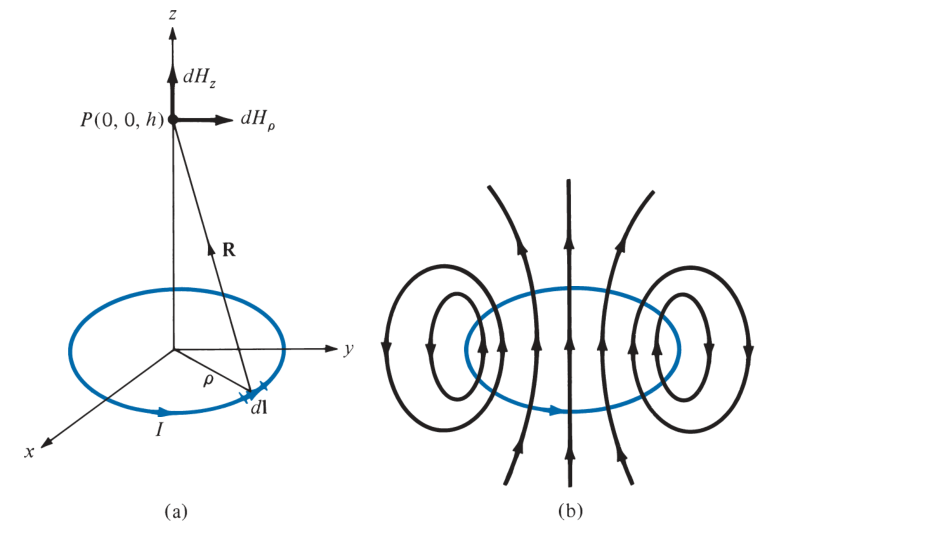
\includegraphics[width=0.85\textwidth]
    {figures/background/Figure_A01.png}
    \caption{Magnetic field around a circular current loop.
    Source: Sadiku \cite{sadiku2018elements}, Fig. 7.8.}
    \label{fig:bg-a01}
\end{figure}

\begin{figure}[htbp]
    \centering
    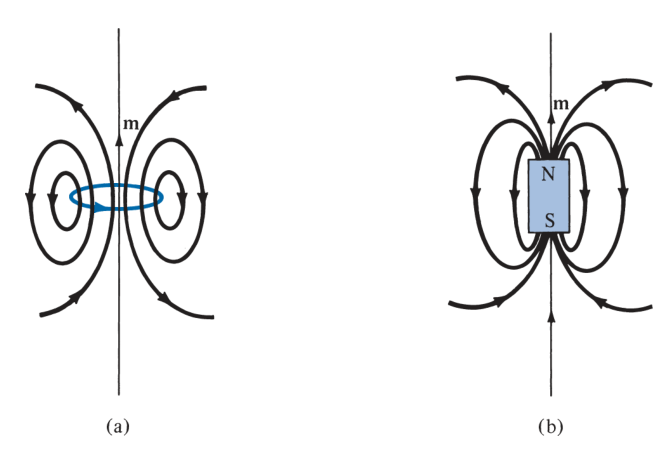
\includegraphics[width=0.85\textwidth]
    {figures/background/Figure_A02.png}
    \caption{Magnetic field of a magnetic dipole.
    Source: Sadiku \cite{sadiku2018elements}, Fig. 8.7.}
    \label{fig:bg-a02}
\end{figure}



\begin{figure}[htbp]
    \centering
    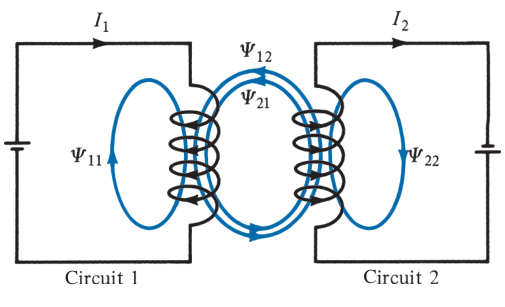
\includegraphics[width=0.85\textwidth]
    {figures/background/Figure_A04.png}
    \caption{Magnetic coupling between two circuits.
    Source: Sadiku \cite{sadiku2018elements}, Fig. 8.20.}
    \label{fig:bg-a04}
\end{figure}





\begin{figure}[htbp]
    \centering
    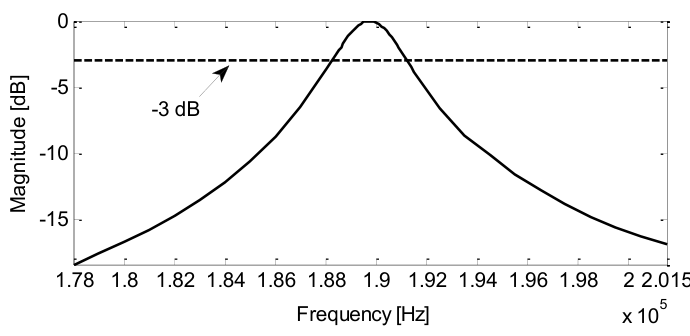
\includegraphics[width=0.85\textwidth]
    {figures/background/Figure_A07.png}
    \caption{Frequency response of the resonant system.
    Source: De Angelis et al.
    \cite{deangelis2015indoor}, Fig. 12.}
    \label{fig:bg-a07}
\end{figure}

\begin{figure}[htbp]
    \centering
    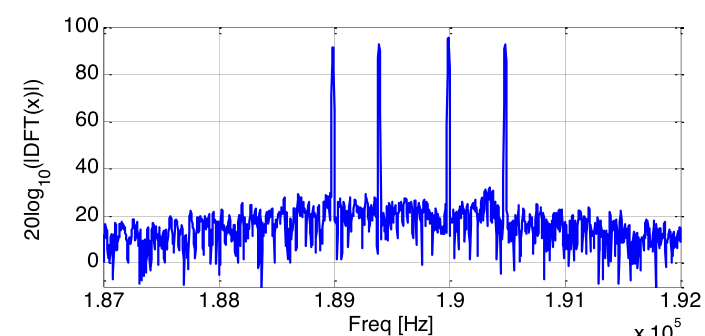
\includegraphics[width=0.85\textwidth]
    {figures/background/Figure_A08.png}
    \caption{Frequency spectrum showing four
    transmitter signals.
    Source: De Angelis et al.
    \cite{deangelis2015indoor}, Fig. 15.}
    \label{fig:bg-a08}
\end{figure}

\begin{figure}[htbp]
    \centering
    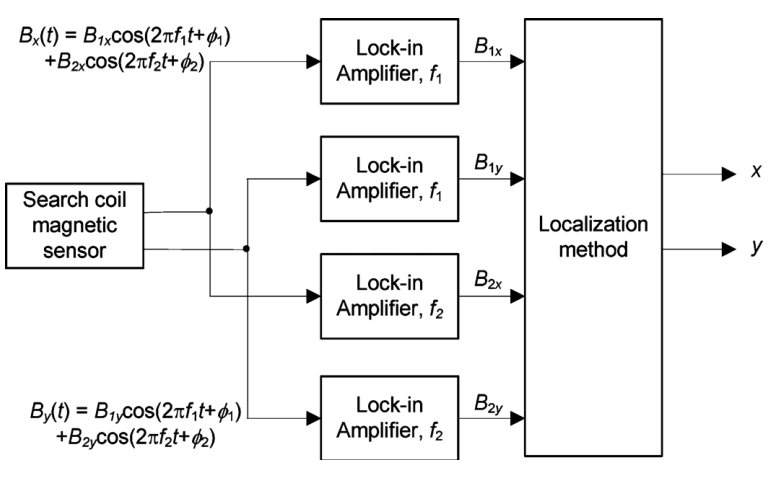
\includegraphics[width=0.85\textwidth]
    {figures/background/Figure_A09.png}
    \caption{Receiver system with four lock-in amplifiers.
    Source: Sheinker et al.
    \cite{sheinker2013localization}, Fig. 2.}
    \label{fig:bg-a09}
\end{figure}

\begin{figure}[htbp]
    \centering
    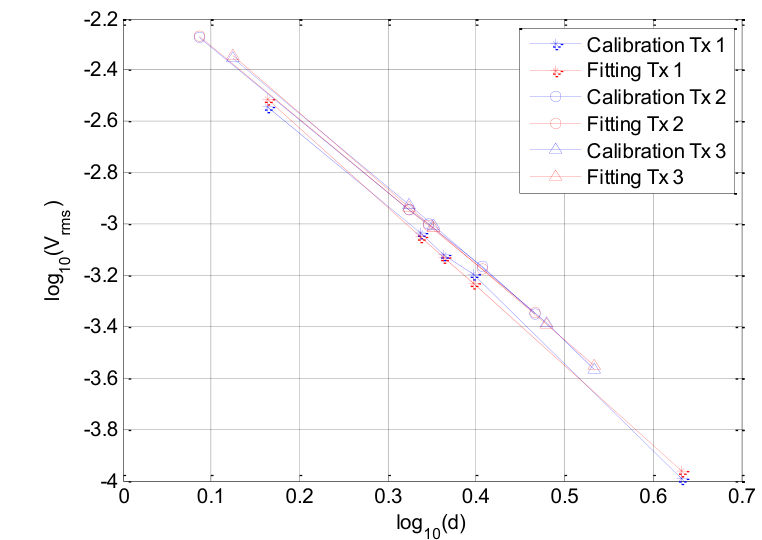
\includegraphics[width=0.85\textwidth]
    {figures/background/Figure_A10.png}
    \caption{Calibration measurements of received
    voltage and distance.
    Source: De Angelis et al.
    \cite{deangelis2015indoor}, Fig. 5.}
    \label{fig:bg-a10}
\end{figure}



\begin{figure}[htbp]
    \centering
    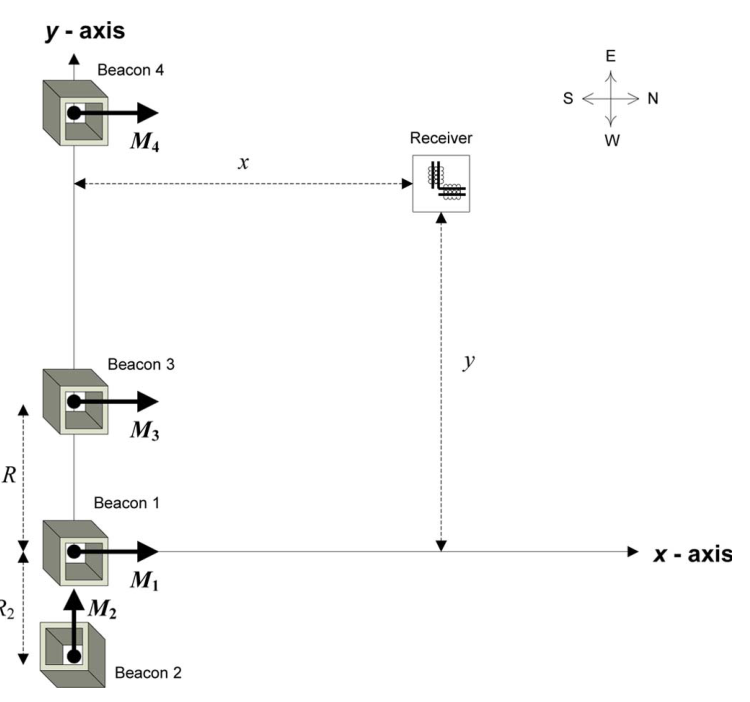
\includegraphics[width=0.85\textwidth]
    {figures/background/Figure_A12.png}
    \caption{Two magnetic beacon arrangements
    for 2D localization.
    Source: Sheinker et al.
    \cite{sheinker2013localization}, Fig. 1.}
    \label{fig:bg-a12}
\end{figure}

\clearpage
